\subsection{Aufbau des Programms}
Das Programm ist in 3 große Teile gegliedert. Dazu zählt das Einlesen der Audiodateien, die benötigte Signalverarbeitung inklusiver Berechnung der gewünschten Parameter und das Speichern der gewonnenen Werte in Form einer Excel-Datei.
\paragraph{Einlesen der Audiodaten}
Die Audiodateien liegen im WAV-Format als Stereoaufnahme vor. Zunächst wird eine Liste mit allen Dateien in einem bestimmten Ordner erstellt, damit die Dateien nacheinander eingelesen werden können. Im nächsten Schritt werden die beiden Kanäle voneinander getrennt, um diese dann in die Signalverarbeitung zu übergeben.
\paragraph{Signalverarbeitung}
Das Kernstück der Signalverarbeitung ist eine periodische Korrelationsfunktion, die den linken und rechten Kanal miteinander korreliert. Die dabei entstandene Korrelationsfunktion wird dann weiter untersucht. Als nächstes wird eine Art Einhüllende berechnet, die ein Maß für die Steilheit der Kurve ist. Wie bereits im Abschnitt 3.3 "Gauß-Regression" beschrieben, wird dann mit Hilfe der Methode der kleinsten Quadrate eine Gauß-Glocke so angepasst, dass sie den Verlauf der Hüllkurve der KKF möglichst gut abbildet. Die Parameter ripple, $\sigma$, Gleichanteil und Zeitverschiebung des Maximums aus dem Ursprung werden danach an eine Funktion übergeben, die diese Daten in einer Excel-Tabelle speichert.
\paragraph{Speicherung}
Die Speicherung der Daten erfolgt in einer Excel-Datei. Dabei wird zu erst der Dateiname des Samples und alles dazugehörigen Werte gespeichert. Außerdem wird noch ein Link zum Graphen der Korrelationsfunktion angegeben, damit man sich diese bei der Auswahl der Test-Signale anschauen kann.

\subsubsection{Programmablaufplan}
\begin{figure}[ht!]
\centering
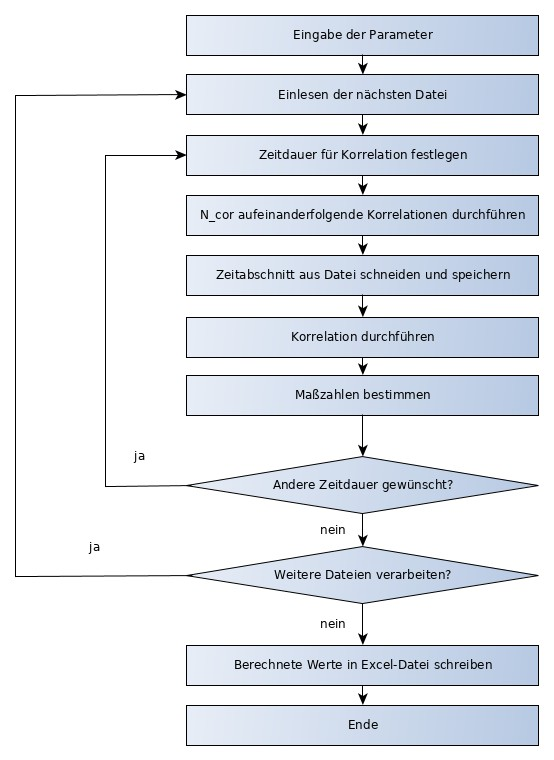
\includegraphics[scale=0.6]{img/pap}
\caption{Programmablaufplan}
\label{figure1}
\end{figure}

\subsection{Mögliche Einstellungen}
Im Code gibt es diverse Eintellungen, die das Verhalten des Programms je nach Wunsch des Anwenders verändern. Diese sind am Beginn der main.m-Datei festgelegt und werden im folgenden beschrieben:
\begin{itemize} 
\item $path$ - Pfad zur Sammlung der WAV-Dateien
\item $excel\_path$ - Pfad unter dem Excel-Datei mit Lösungen gespeichert wird
\item $output$ - Unterscheidung, ob Ergebnisse gespeichert oder angezeigt werden
\item $calc$ - Wechsel zwischen Berechnung im Zeit- und Frequenzbereich möglich.
\item $x\_axes$ - Unterscheidung, ob Korrelation gegen Samples oder Zeit aufgetragen wird
\item $priority$ - Unterscheidung, ob angegebene Blocklänge oder Zeitdauer priorisiert wird
\item $t\_start$ - Startzeitpunkt der Korrelation
\item $t\_dur$ - Array $A1$ mit Menge an Zeitdauern die korrelierten werden sollen, Korrelation beginnt immer bei $t\_start$
\item $Ncor\_init$ - Array, mit identischer Länge zu $A1$. Gibt an wie oft korrespondierender Eintrag in $A1$ hintereinander korreliert wird. 
\item $Lcor$ - Blocklänge der Korrelation
\end{itemize}
\subsection{Probleme} 
Zu Beginn unserer Arbeit wurde die Korrelation zuerst in Python implementiert. Allerdings nahm die Berchnungsdauer mit zunehmende Blocklänge stark zu. Da die .wav Dateien mit 44100Hz abgetastet werden werden die zu berechnenden Summen schnell sehr groß. Wie in der Theorie und im Abschnitt zur Software schon erklärt, wird nun Octave und der Fouriertransformation genutzt. \\\\Darauf aufbauen war noch die Problemstellung der Bemessung der korrelierten Signale zu lösen. Dabei mussten Maßzahlen entstehen, die viele verschiedene Faktoren beachteten und möglichst gute Aussagen über "Piekigkeit" und Streuung der KKF trafen. Die Idee war dann ein Fit mit einer Funktion wie der Gauß-Kurve, die als Parameter schon eine Verteilung beinhaltet.Allerdings ist die KKF nach der Berechnung sehr "eckig" und weißt viele Nullstellen auf. Um den Fit nicht durch diese Eigenschaften verzerren zu lassen, wird die KKF durch einen Tiefpass gefiltert. Auf die geglättete Kurve angewendet, ist die angewendete Regression aussagekräftiger.